\printMiniToc

\label{chap:gameplay}

\normalInfo{Une question de vocabulaire}{Ce chapitre porte sur un sujet relativement technique et récent. L'univers du jeu vidéo étant principalement anglophone, le vocabulaire de ce domaine est composé de beaucoup d'anglicismes, tel \anglicisme{gameplay}. La langue française n'a pas encore eu le temps de s'adapter. Pour cette raison, les anglicismes seront conservés et typographiés de \anglicisme{cette façon}.}

\section{Idée générale}
Ce jeu tente de promouvoir la paix et la résolution de problème par des solutions non-violentes. De ce parti pris découleront bien des aspects. Ainsi, le joueur sera \enquote{puni} s'il utilise ses armes, mais il est à noter qu'elles restent à disposition et peuvent être améliorées, tout comme d'autres items. C'est aussi une question qui est posée au joueur: quelle voie préfère-t-il utiliser? Pacifique ou brutale? Libre à lui de choisir, mais le jeu prend parti pour celle qui n'utilise pas la violence et répercute cela sur le score et certaines ressources.

\section{Mode de jeu \anglicisme{stealth}}
\anglicisme{Stealth}, en français, peut se traduire par furtif, discret, ruse ou encore dissimulation. Dans les milieux francophones, on parlera de jeu d'infiltration à la place de \anglicisme{stealth game}, cependant le sens n'est pas exactement le même. Ce terme, sans bonne traduction, représente bien le style de gameplay que l'on peut rencontrer dans \nomJeu. Le jeu défendant une approche pacifique, il est bien sûr hors de question de faire tirer le joueur sur ses ennemis ou de lui permettre de les démolir à coups de poings ou d'épée.

À la place, c'est un mode de jeu où il faut éviter les opposants, se cacher et rester discret, qui est privilégié. Un autre aspect développé est la résolution de problèmes, ainsi que la complétion de sous-quêtes. Finalement, on notera l'utilisation relativement répandue de puzzles\definition, qui nécessiteront de collecter des objets au fil des aventures pour pouvoir être résolus (\anglicisme{item collecting}). \cite{Stealthgame_}


\section{Les ressources}
Un élément important dans les jeux vidéos est représenté par les ressources. Des exemples de ressources sont l'argent, l'expérience (souvent abrégée XP), les munitions ou encore le mana qui représente une quantité de magie. Elles forment le \enquote{système économique}. La mesure dans laquelle les ressources sont disponibles peut faire toute la différence entre un bon et un mauvais titre: si elles sont trop abondantes, le jeu devient facile et les joueurs perdent leur intérêt, à l'inverse, si elles sont trop rares et difficiles à obtenir, le joueur se retrouve confronté à une difficulté trop importante et cesse de joueur par dépit.\cite{LevelUpTheGuidetoGreatVideoGameDesign_Rogers}

Dans \nomJeu, les ressources principales sont les suivantes:
\begin{itemize}
	\item Argent
	\item Énergie verte
	\item Coefficient de naturalité (score)
	\item Graines
\end{itemize}

L'énergie verte est une ressource un peu spéciale. Elle est décrite dans la section \ref{sec:energieTelurans} du point de vue de l'univers. Dans le jeu, elle est principalement utilisée pour lancer des sorts.

Les graines sont un autre type de ressource. Ces dernières sont rares et dispersées dans le jeu. Toutes les fonctionnalités décrites ci-après sont accessibles dans un menu séparé en 2D. Lorsque le joueur en découvre ou gagne une, il peut la planter. Il doit ensuite l'arroser et la nourrir. Plus il entretient la plante, plus elle grandit vite. Une fois adulte, la plante donne des fruits que le joueur peut cueillir, ce sont des bonus de vie, d'énergie verte, des ingrédients, etc. La quantité de fruits qui poussent dépend de l'attention apportée à la plante.

Les succès\definition\ font aussi partie du système économique mais pas au même titre que les ressources précédemment citées. En effet, on ne peut que gagner ou débloquer un succès, à l'accomplissement d'objectifs supplémentaires par exemple; impossible de les utiliser ou de les vendre ensuite. Ils font cependant partie du système de récompenses.

\begin{table}[ht!]
	\begin{tabu} to \textwidth {l X X[1.2] X[1.2] l}
		\rowfont{\fontspec{Lato Heavy}\selectfont\leavevmode\color{white}}
		\rowcolor{mainColor}
		& Ressources principales & Comment en gagner & Comment en perdre & \\
		& Argent & Compléter des quêtes,\newline Dans les coffres & Achats & \\
		& Énergie verte & Planter une graine,\newline Se régénère avec le temps & Utiliser la violence,\newline Lancer un sort & \\
		& Coefficient de naturalité & Faire preuve de naturalité,\newline Compléter des sous-quêtes & Utiliser la violence & \\
	\end{tabu}
	\caption{Gestion des ressources principales}
\end{table}

\section{Les sorts}
\label{sec:sorts}
Les sorts sont les principaux outils mis à la disposition du joueur.

Dans l'univers d'\nomUnivers, pour pouvoir lancer un sort, il faut posséder, le totem qui lui est associé. Ces totems se présentent sous la forme de petits grigris. Les esprits sont les seules créatures qui peuvent offrir de tels artéfacts. Chaque esprit possède trois totems qui lui sont propres. Il y a donc un total de neuf sorts majeurs. Ces sorts sont coûteux en énergie verte, mais nécessaires pour avancer dans l'histoire.

Les sorts mineurs en revanche ne nécessitent pas de totem. On peut découvrir des parchemins expliquant comment les lancer un peu partout dans l'univers et ils ont besoin de nettement moins d'énergie verte pour pouvoir être lancés.


\section{Les objets}
Les objets sont un élément important du jeu dans le sens qu'ils permettent au joueur d'interagir avec l'environnement virtuel. Gagner un nouvel objet sera souvent la clé pour terminer un niveau, car il permettra d'accéder à de nouveaux endroits, de débloquer certains passages, etc. Le joueur pourra s'équiper de deux objets à la fois et passer très rapidement de l'un à l'autre à l'aide de touches de raccourcis. Pour changer les objets dont il sera équipé, il devra passer par le menu.

\newpage
\subsection{Bâton de bois}
\warningInfo{Objet le plus important}{Le bâton de bois est sans conteste l'objet le plus utile et le plus important. Il est le catalyseur nécessaire pour lancer des sorts. Ces pouvoirs sont sans aucun doute le moyen d'interaction le plus puissant conféré au joueur.}

C'est sur le bâton de bois qu'il faut placer les totems représentant les sorts afin de les activer. Il pourra, de plus, être personnalisé par l'ajout de runes (dont la couleur pourra être spécifiée) ou par l'ajout de décorations (débloquées grâce aux succès). Le bâton pourra aussi être amélioré: au début du jeu, il ne peut porter, au maximum, que trois totems, mais cette valeur peut être augmentée au fil des niveaux. C'est un item particulièrement intéressant du gameplay, car il offre au joueur la possibilité de personnaliser un objet, et met en avant les succès du joueur. Ce dernier se sentira alors d'autant plus impliqué, ce qui le motivera à poursuivre le jeu.

\begin{figureWithNotes}[ht!]
	\center
	\subfloat[\label{subfig:batonBoisSimple}Bâton de bois simple]{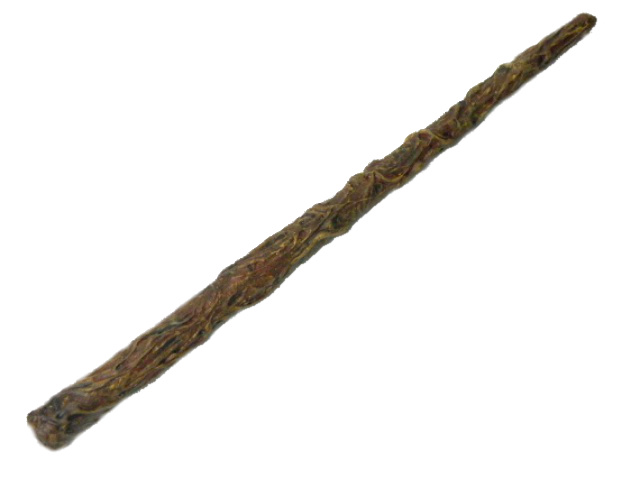
\includegraphics[width=.48\linewidth]{images/Gameplay/batonBoisSimple.jpg}}
	\hspace*{.04\linewidth}
	\subfloat[\label{subfig:batonBoisRune}Bâton de bois avec des runes décoratives et deux totems]{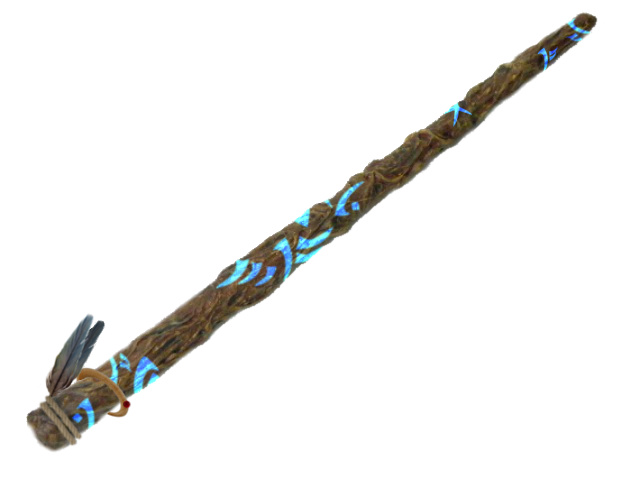
\includegraphics[width=.48\linewidth]{images/Gameplay/batonBoisRune.jpg}}
	
	\caption{Esquisse du bâton de bois {\cite{Baguettemagique_}}\label{fig:batonBois}}
\end{figureWithNotes}

\subsection{Sarbacane}
La sarbacane est un objet qui permet de tirer au loin de petites fléchettes. Cela ajoute une nouvelle distance, plus éloignée, au gameplay. Les fléchettes et leur éventuel contenu doivent être créés par le joueur. Il doit ainsi trouver le bois nécessaire aux dards (disponible en grande quantité, là ne réside pas le problème) mais surtout les recettes et ingrédients pour fabriquer les poisons à insérer dans les projectiles. À ce moment, le joueur peut créer des mixtures mortelles, soporifiques, empoisonnées, etc. L'idée derrière cet objet, le deuxième plus important du jeu, est de permettre au joueur de choisir entre une résolution de conflit \enquote{pacifique} ou meurtrière.

Pour le joueur, les recettes de poison sont de nouvelles récompenses et les ingrédients, éparpillés dans l'univers, devront être collectionnés (\anglicisme{item collecting}) afin de pouvoir finalement réaliser la potion désirée.


